Existen números herramientas de etiquetado compatibles con \textbf{YOLO}, pero quizás una de las más sencillas de usar sea \textit{LabelIMG}. Esta herramienta se encuentra disponible tanto para \textit{Windows} como para \textit{MAC OS/Linux}.\\

Para poder acceder a \textit{LabelIMG} se puede hacer a través de su propio repositorio de \textit{GitHub} \url{https://github.com/heartexlabs/labelImg}, el cual presenta las distintas opciones de instalación que se tienen dependiendo de la plataforma. En caso de necesitar instalarla en un ordenador \textit{MAC OS/Linux}, debido a las diferentes incompatibilidades entre librerías con las que nos encontramos en su momento, recomendamos instalar las que se indican en el fichero de \textbf{requirements.txt}. \\

Para hacer uso de dicha herramienta simplemente debemos inicializar su fichero base, el cual lanzará una interfaz con la que interactuaremos para realizar el etiquetado. Para ello, accediendo a la segunda carpeta de nuestro repositorio denominada \textit{2_Etiquetado}, podremos arrancarla:

\begin{lstlisting}
python3 labelImg.py
\end{lstlisting}

Internamente podemos modificar cuáles queremos que sean las clases que por defecto tenemos para etiquetar, en nuestro caso tenemos las diferentes clases de señales: prohibición, peligro, obligación y otros. Si se quisiera modificarlo porque se fuera a utilizar para otra aplicación, se podría modificar mediante el fichero \textbf{predefined_classes.txt} disponible dentro de la carpeta \textit{data}.\\

Se puede trabajar con una imagen individual o con un conjunto de ellas, a través de los botones indicados a continuación podremos abrir las imágenes:

\begin{figure}[H]
	\centering
	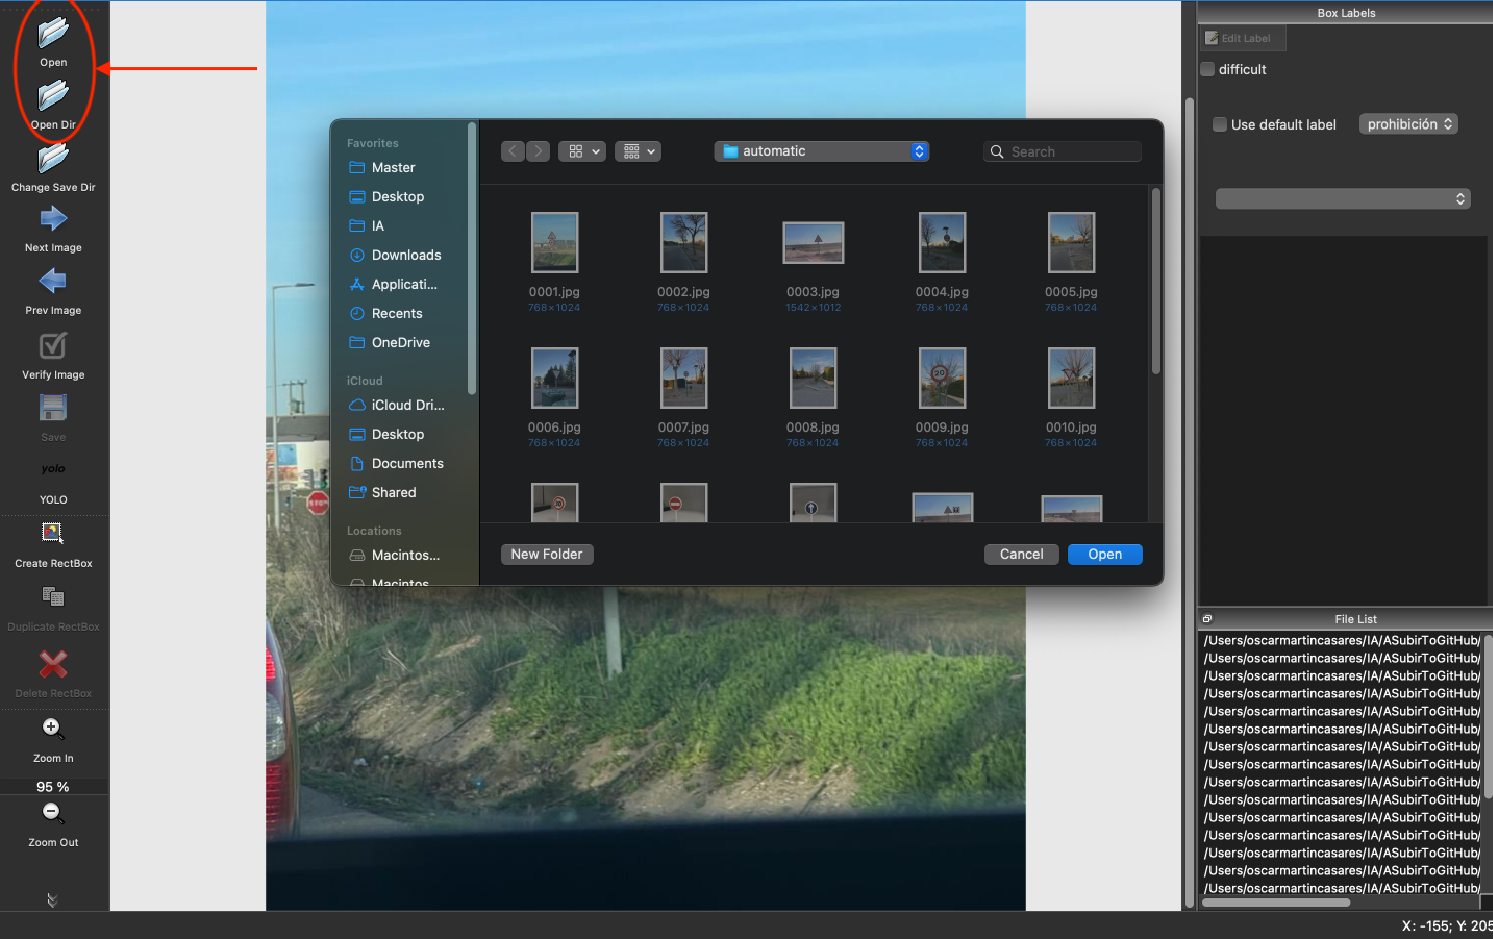
\includegraphics[width=\textwidth]{Imagenes/AnexoI_Manual/AA/etiquetado1.pdf}
	\caption{Etiquetado de una señal}
	\label{etique1}
\end{figure}

Debemos asegurarnos de que el formato en el que se va a producir el etiquetado debe ser únicamente \textbf{YOLO} (ver figura \ref{etique2}. Pulsando sobre el icono mostrado podremos ir intercambiando entre diferentes formatos, ya que esta herramienta es compatible con varios.\\

\begin{figure}[H]
	\centering
	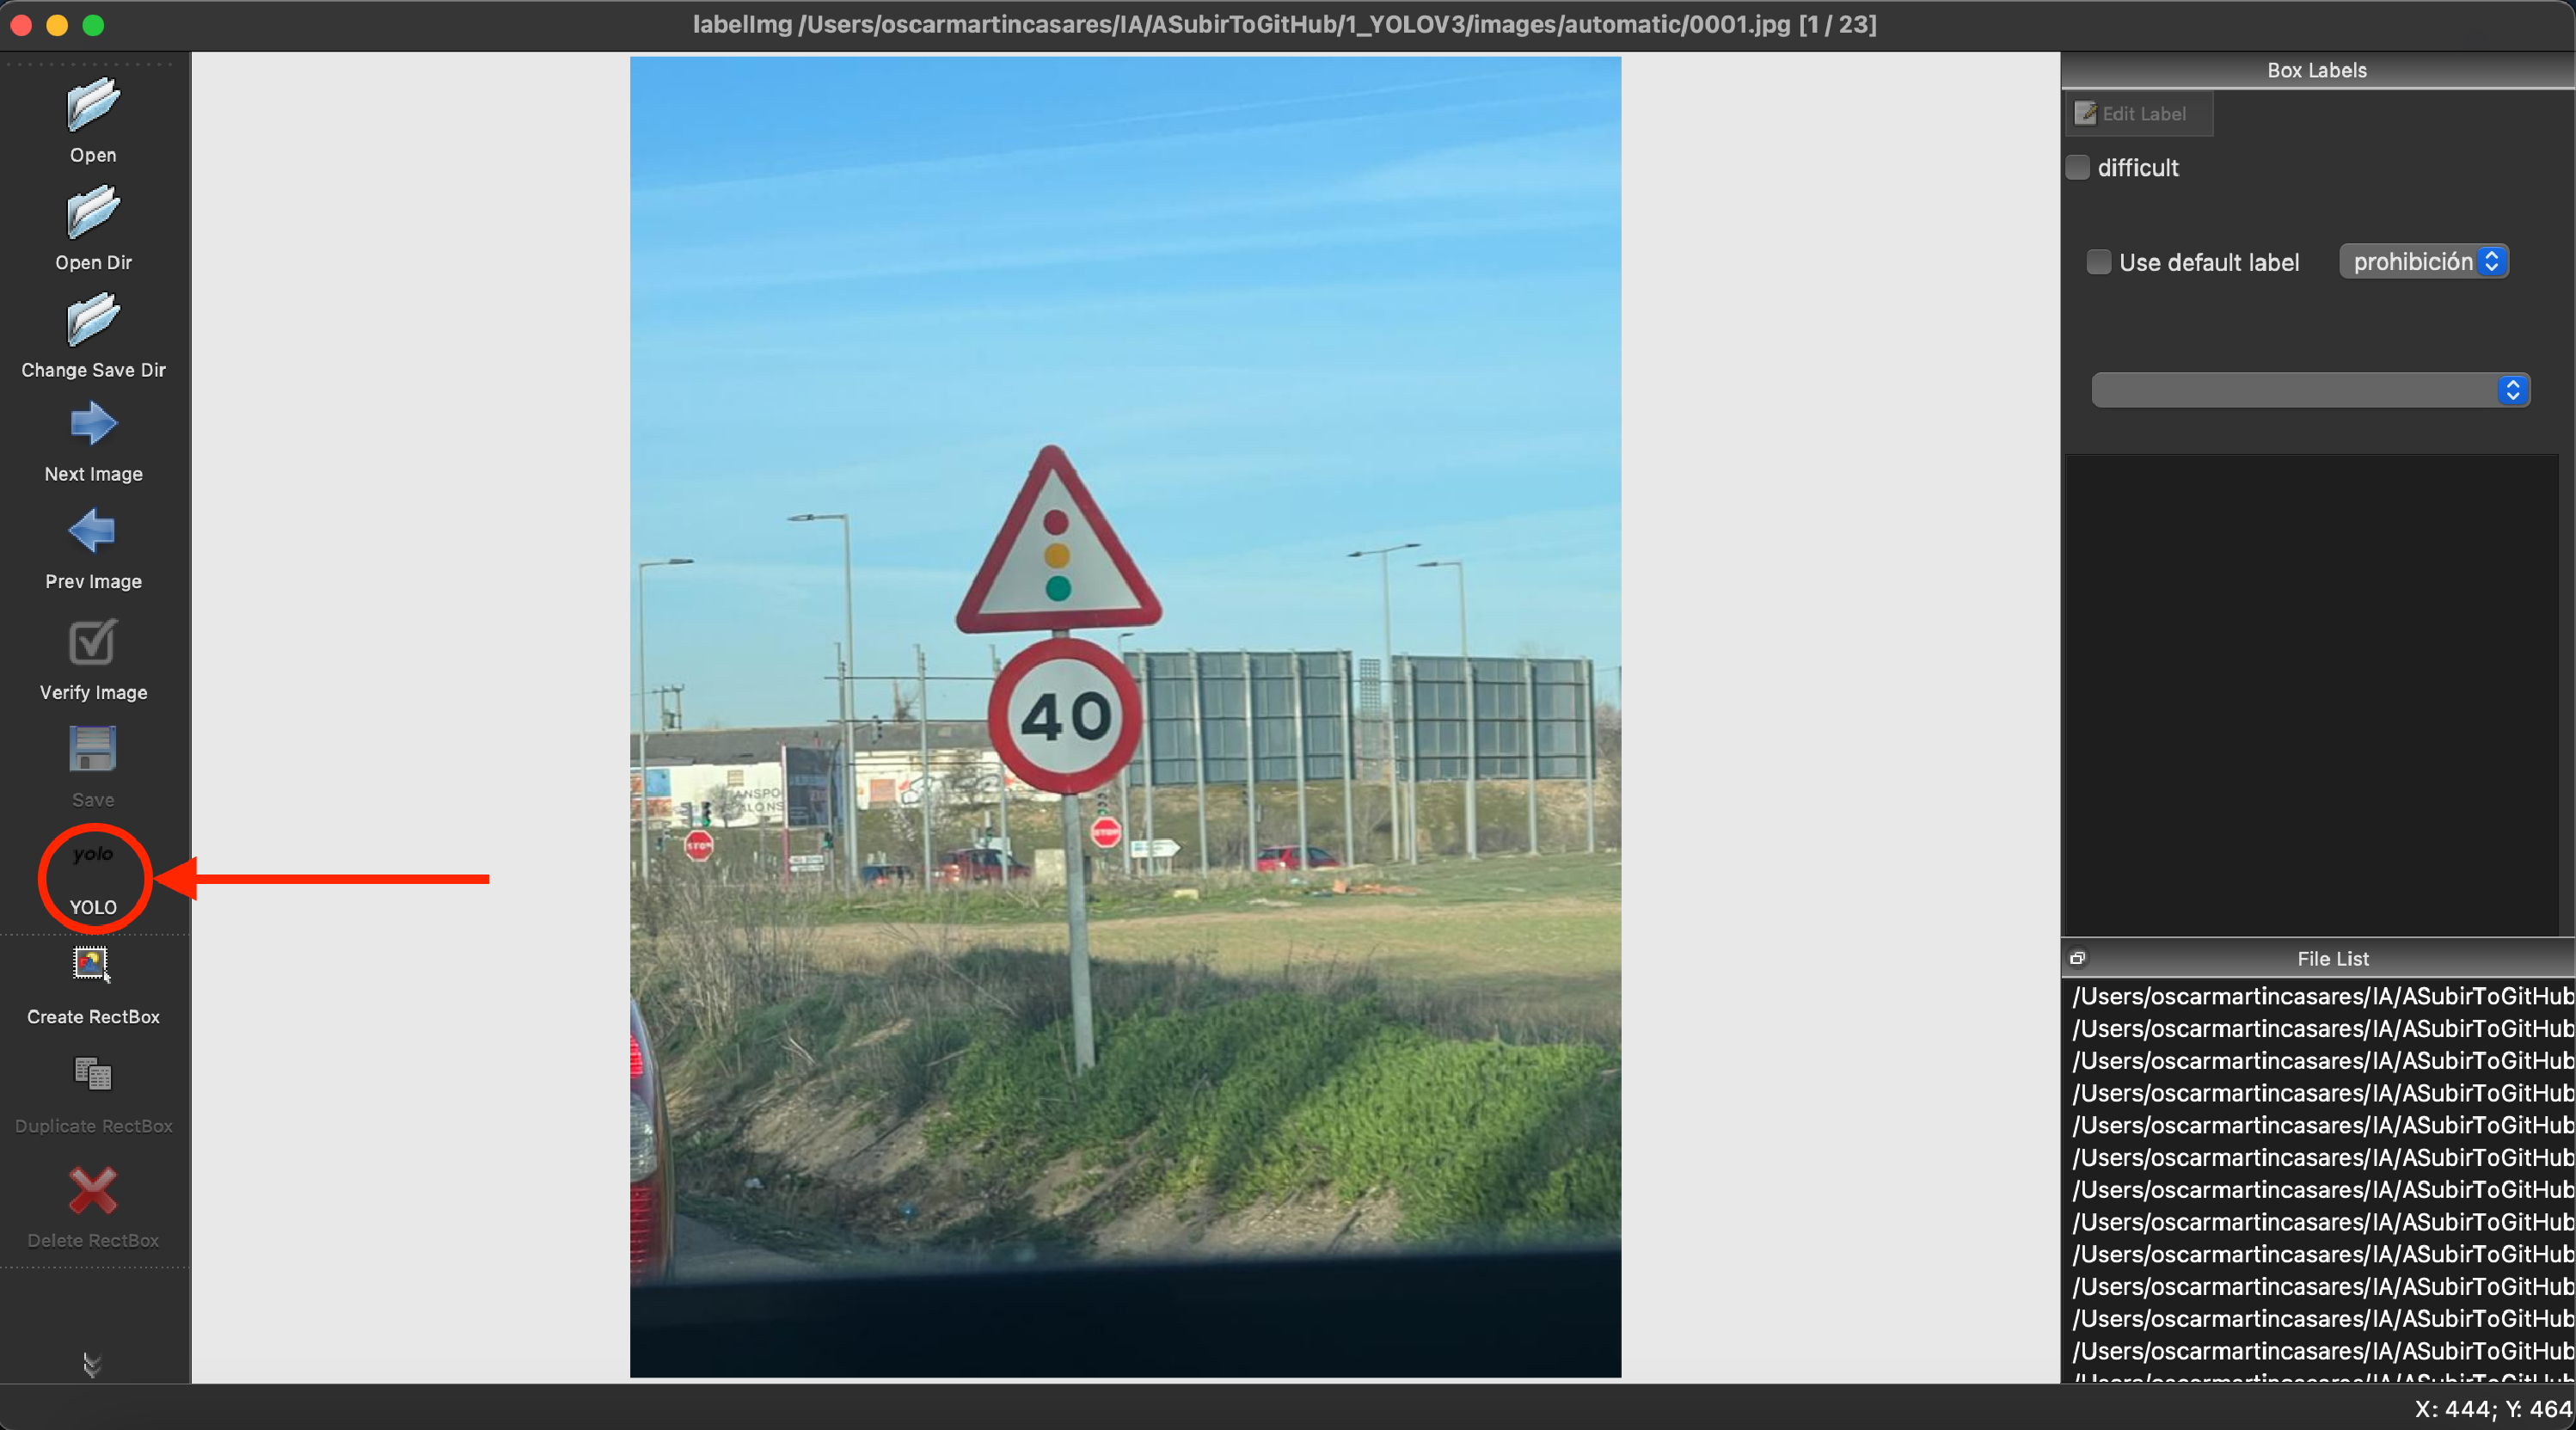
\includegraphics[width=\textwidth]{Imagenes/AnexoI_Manual/AA/etiquetado2.pdf}
	\caption{Selección del modelo}
	\label{etique2}
\end{figure}

Y mediante la opción \textit{Create RectBox} podremos crear los cuadros delimitadores o \textit{bounding boxes} indicando de qué tipo de señal se trata. Ver en la figura \ref{etique3}


\begin{figure}[H]
	\centering
	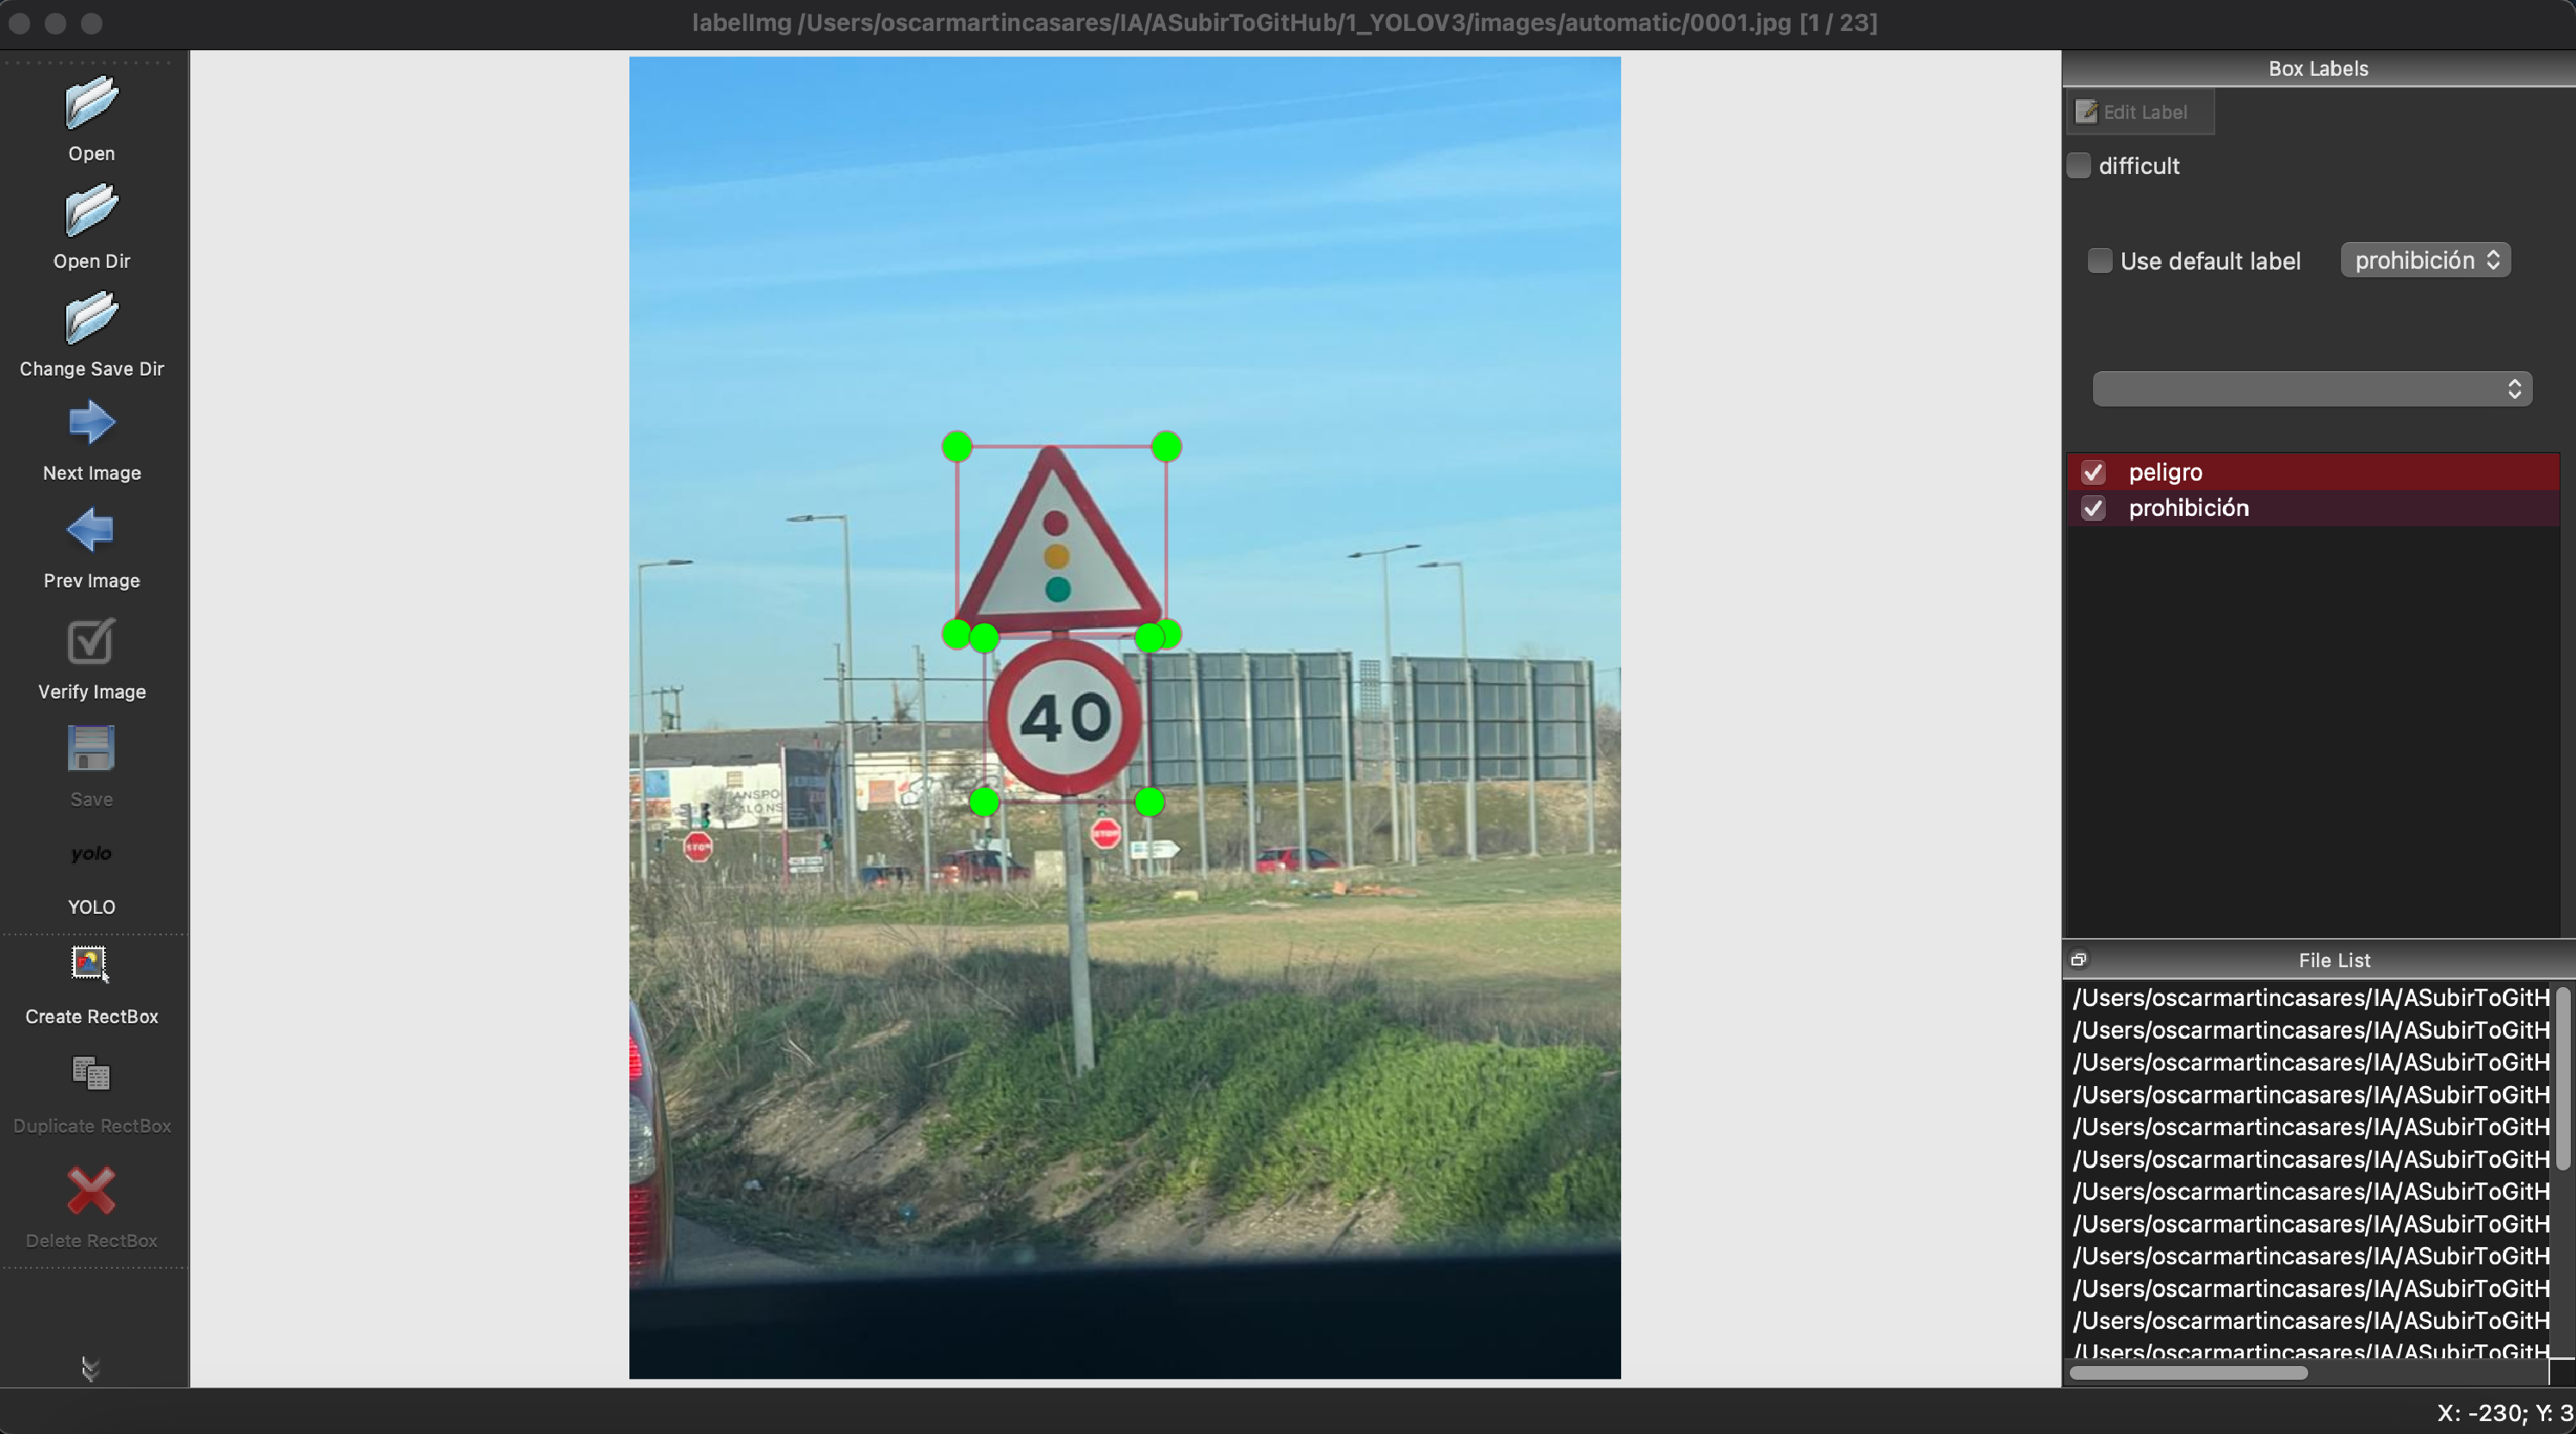
\includegraphics[width=\textwidth]{Imagenes/AnexoI_Manual/AA/etiquetado3.pdf}
	\caption{Cuadros delimitadores}
	\label{etique3}
\end{figure}

Al guardar la imagen se nos creará un fichero en formato \textbf{TXT} que contendrá la información de etiquetado (Figura \ref{etique4}) en el directorio que contenga la imagen en cuestión, con idéntico formato \textbf{YOLO} a como se nos mostraba en detección con la opción \textit{medirRendimientoRed} a \textbf{True}.

\begin{figure}[H]
	\centering
	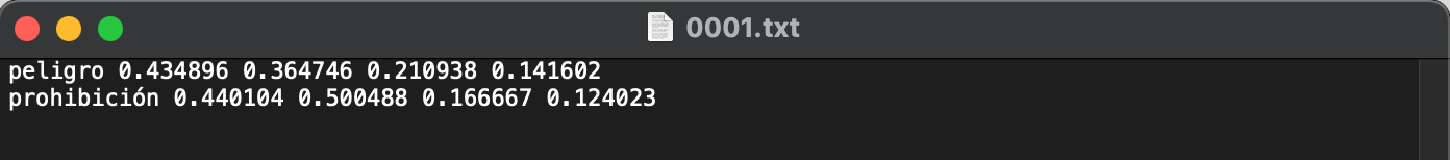
\includegraphics[width=\textwidth]{Imagenes/AnexoI_Manual/AA/etiquetado4.pdf}
	\caption{Fichero con la información de etiquetado}
	\label{etique4}
\end{figure}

Además, creemos de puede ser de utilidad una herramienta que convierta un video a \textit{frames}, para poder etiquetarlos de manera manual para entrenar o cualquier otra aplicación. Esta herramienta se llama \textbf{ffmpeg} \url{https://ffmpeg.org} y se puede instalar de manera muy sencilla mediante el comando: 

\begin{lstlisting}
pip3 install ffmpeg 
\end{lstlisting}

Simplemente desde línea de comandos podremos utilizarla, indicando cuál es el video que queremos dividir, en cuántos \textit{frames} queremos dividirlo y cómo queremos que se llamen cada una de las imágenes. 

\begin{lstlisting}
ffmpeg -i nombre_video.mp4 -vf fps=4 nombre_imagen-%d.jpeg
\end{lstlisting}
